\documentclass[12pt, twocolumn, landscape, a4paper]{article}

\usepackage[margin=1in]{geometry}
\usepackage[utf8]{inputenc}
\usepackage{babel}
\usepackage{amssymb, amsmath, amsbsy}
\usepackage{verbatim}
\usepackage{bookman}
\usepackage{enumerate}
\usepackage{tikz}
\usetikzlibrary{angles,quotes}
\usepackage[pdftex]{hyperref}
\hypersetup{ pdftitle = {   },pdfauthor = {Luis Carrillo Gutiérrez} }

\renewcommand{\familydefault}{\sfdefault}

\begin{document}
\section*{Adición de fuerzas}
La suma de dos o más vectores fuerza es otro vector denominado \textbf{vector fuerza resultante} ($\vec{F}_{R}$). Para sumar dos o más vectores fuerza, se deben ubicar estos, uno a continuación de otro; el vector fuerza resultante será aquel que parte del origen del primer vector y llega al extremo del último vector. \\

\noindent Ejemplos : Sumar las fuerzas en los siguientes casos : \\

\begin{enumerate}[a)]
\item{
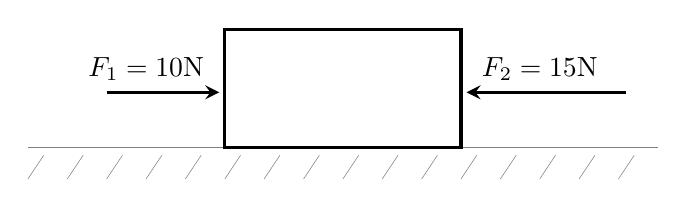
\begin{tikzpicture}
	% \coordinate () at ();
	\draw[gray, very thin] (-4, 0) -- (4, 0);
	\draw[line width =1.2pt] (-1.5, 0) -- (-1.5, 1.5) -- (1.5, 1.5) -- (1.5, 0) -- cycle;
	\draw[line width =1.2pt, ->, >=stealth] (-3, .7) -- (-1.57, .7);
	\draw[line width =1.2pt, ->, >=stealth] (3.6, .7) -- (1.57, .7);
	\draw (-2.5, 1) node{$F_{1} = 10\mathrm{N}$};
	\draw (2.5, 1) node{$F_{2} = 15\mathrm{N}$};
	
	\foreach \time in {-4,...,3} {
		\draw[gray, very thin] (\time + .2, -.1) -- (\time, -.4);
		\draw[gray, very thin] (\time + .7, -.1) -- (\time + .5, -.4);
	}
\end{tikzpicture}
}
\item{
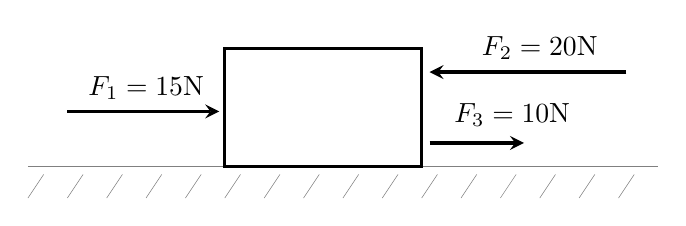
\begin{tikzpicture}
	% \coordinate () at ();
	\draw[gray, very thin] (-4, 0) -- (4, 0);
	\draw[line width =1.2pt] (-1.5, 0) -- (-1.5, 1.5) -- (1, 1.5) -- (1, 0) -- cycle;
	\draw[line width =1.2pt, ->, >=stealth] (-3.5, .7) -- (-1.57, .7);
	\draw[line width =1.2pt, ->, >=stealth] (3.6, 1.2) -- (1.1, 1.2);
	\draw[line width =1.2pt, ->, >=stealth] (1.1, .3) -- (2.3, .3);
	\draw (-2.5, 1) node{$F_{1} = 15\mathrm{N}$};
	\draw (2.5, 1.5) node{$F_{2} = 20\mathrm{N}$};
	\draw (2.15, .65) node{$F_{3} = 10\mathrm{N}$};
	
	\foreach \time in {-4,...,3} {
		\draw[gray, very thin] (\time + .2, -.1) -- (\time, -.4);
		\draw[gray, very thin] (\time + .7, -.1) -- (\time + .5, -.4);
	}
\end{tikzpicture}
}
\end{enumerate}
% \begin{comment} \end{comment}
\end{document}